\label{sec:rocking_curve_section}
Весьма наглядной иллюстрацией являются собственные кривые отражения от Si(440) рассчитанные при
трех разных углах падения и соответсвенно имеющие разный коэффициент асимметрии. Угол
Брэгга для такой плоскости отражения составляет $\theta_B = 21.68^o$, угол наклона поверхности
составляет $\varphi = 20^o 53^{'}$.

\begin{figure}[H]
\centering
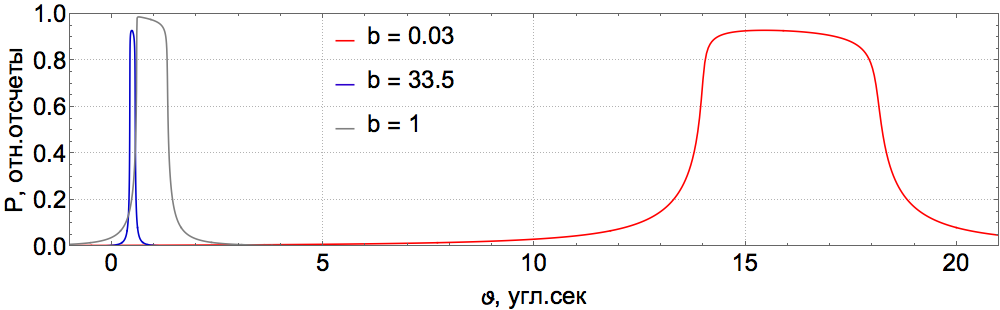
\includegraphics[width=0.99\textwidth]{images/rocking_curve_assym_3.png}
\caption{Кривые отражения 440 $MoK_{\alpha 1}$ от Si, полученные при разных углах падения(для разных b)}
\label{ris:rocking_curve_assym_3}
\end{figure}
Сдвиг центра кривой происходит из-за наличия преломления на величину 0.5 и 16.5 угловых секунд.

% Варьируя угол между поверхностью кристалла и отражающей плоскостью (например, с помощью шлифовки),
% можно существенно изменить ширину рентгеновского пучка (рис. ~\ref{ris:assym_width_beam}).
% \begin{figure}[H]
%  \centering
%  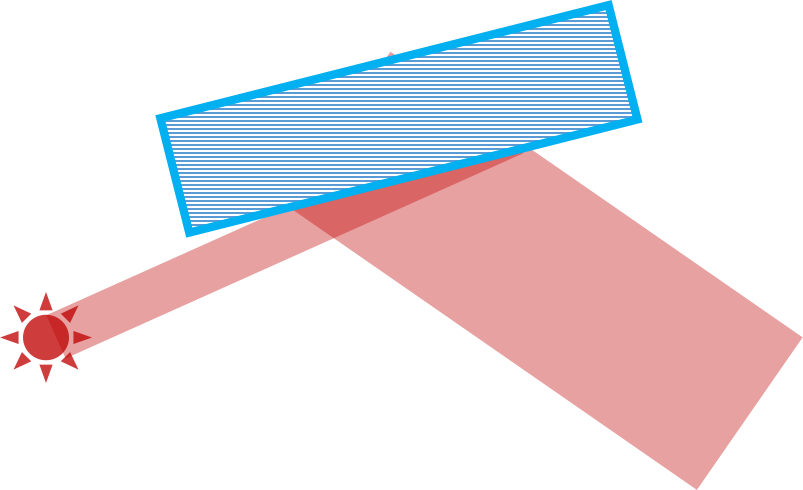
\includegraphics[width=0.4\textwidth]{images/assym_width_beam.png}
%  \caption{Кристалл с асимметричным отражением по Брэггу}
%  \label{ris:assym_width_beam}
% \end{figure}
